\section{Background (Arun)}
\label{sec:background}

[\textbf{FIXME} Need to decide if we want to mention agentic flow for architectural phase]

%%% ------------------------
%%% Agentic-AI Generative HW
%%% ------------------------
\subsection{Agentic-AI Generative Hardware}

Once the architecture is finalized, the components are described using a hardware description language such as Verilog and the design undergoes verification. 

[\textbf{FIXME} Discuss and write this section...]

After verification, the hardware model is transformed into a manufacturable layout using a series of tools outlined in the following section.

%%% ------------------------
%%% RTL-to-GDS Design Flow
%%% ------------------------
\subsection{RTL-to-GDS Design Flow}

%%% FIGURE: RTL-TO-GDS Desing Flow 
%%% ------------------------
\begin{figure}[htbp]
	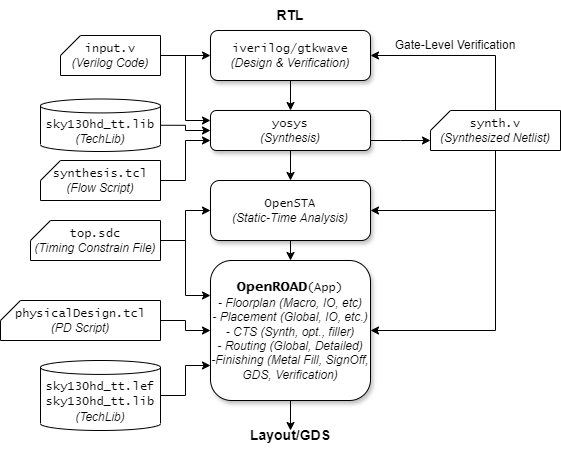
\includegraphics[width=0.45\textwidth]{figs/rtl2gds-toolchain.png}
	\caption{RTL-to-GDS design flow using open-source tools.}
	\label{fig:RTL-to-GDS}
\end{figure}

After the design has been verified and finalized, physical design tools are employed to transform the abstract hardware model into its physical form (GDSII). Figure~\ref{fig:RTL-to-GDS} illustrates a physical design flow utilizing a chain of open-source tools. The first step in the physical design (PD) process is \textit{synthesis}, where a tool like \textit{Yosys} synthesizes the Verilog description into a lower-level representation, such as a netlist of logic gates, suitable for physical implementation. In addition to the Verilog design code, Yosys also requires a technology library (\texttt{*.lib}) and a command script (	\texttt{*.tcl}) to perform the synthesis of the Verilog design. Once synthesis is completed, verification usually involves two steps: 1) 	\textit{Formal verification} or gate-level simulation to confirm that the synthesized netlist's functionality aligns with the original Verilog model; 2) Static Timing Analysis (STA) to ensure there are no timing issues across various process corners and temperature conditions. 
The widely adopted tool for Static Timing Analysis (STA) is the open-source software \textit{OpenSTA}. The input to OpenSTA is the synthesized netlist and a timing constrained file (\texttt{*.sdc}). 
After verifying that the timing requirements are met, the physical design is completed using a leading open-source application \textit{OpenROAD} \cite{ajayi2019toward}\cite{ajayi2019openroad}.
OpenROAD itself contains many complex steps including floorplanning, cell placement, clock-tree synthesis (CTS), routing and finishing steps. In addition, every step involves several substeps, which vary depending on the complexity of the design. Each step utilizes tools and scripts, predominantly written in \textit{Tcl}, to automate the workflow. 

[\textbf{FIXME}: Should we add details of each flow ?]

While OpenROAD aims for "RTL-to-GDS in 24-hours with No-Human-in-Loop (NHIL)", it nevertheless requires a specialist in digital physical design to initiate and manage the flow, and human intervention is still needed to resolve any flow or design issues.
Furthermore, almost every step mentioned calls for \textit{ timing closure}, and an expert usually handles error corrections manually.

[\textbf{FIXME}: Write how agentic flow can integrate into the flow assisted physical design flow for a medium level expert in this field ?]

